\subsection{Design}

\begin{figure}[h]
    \centering
    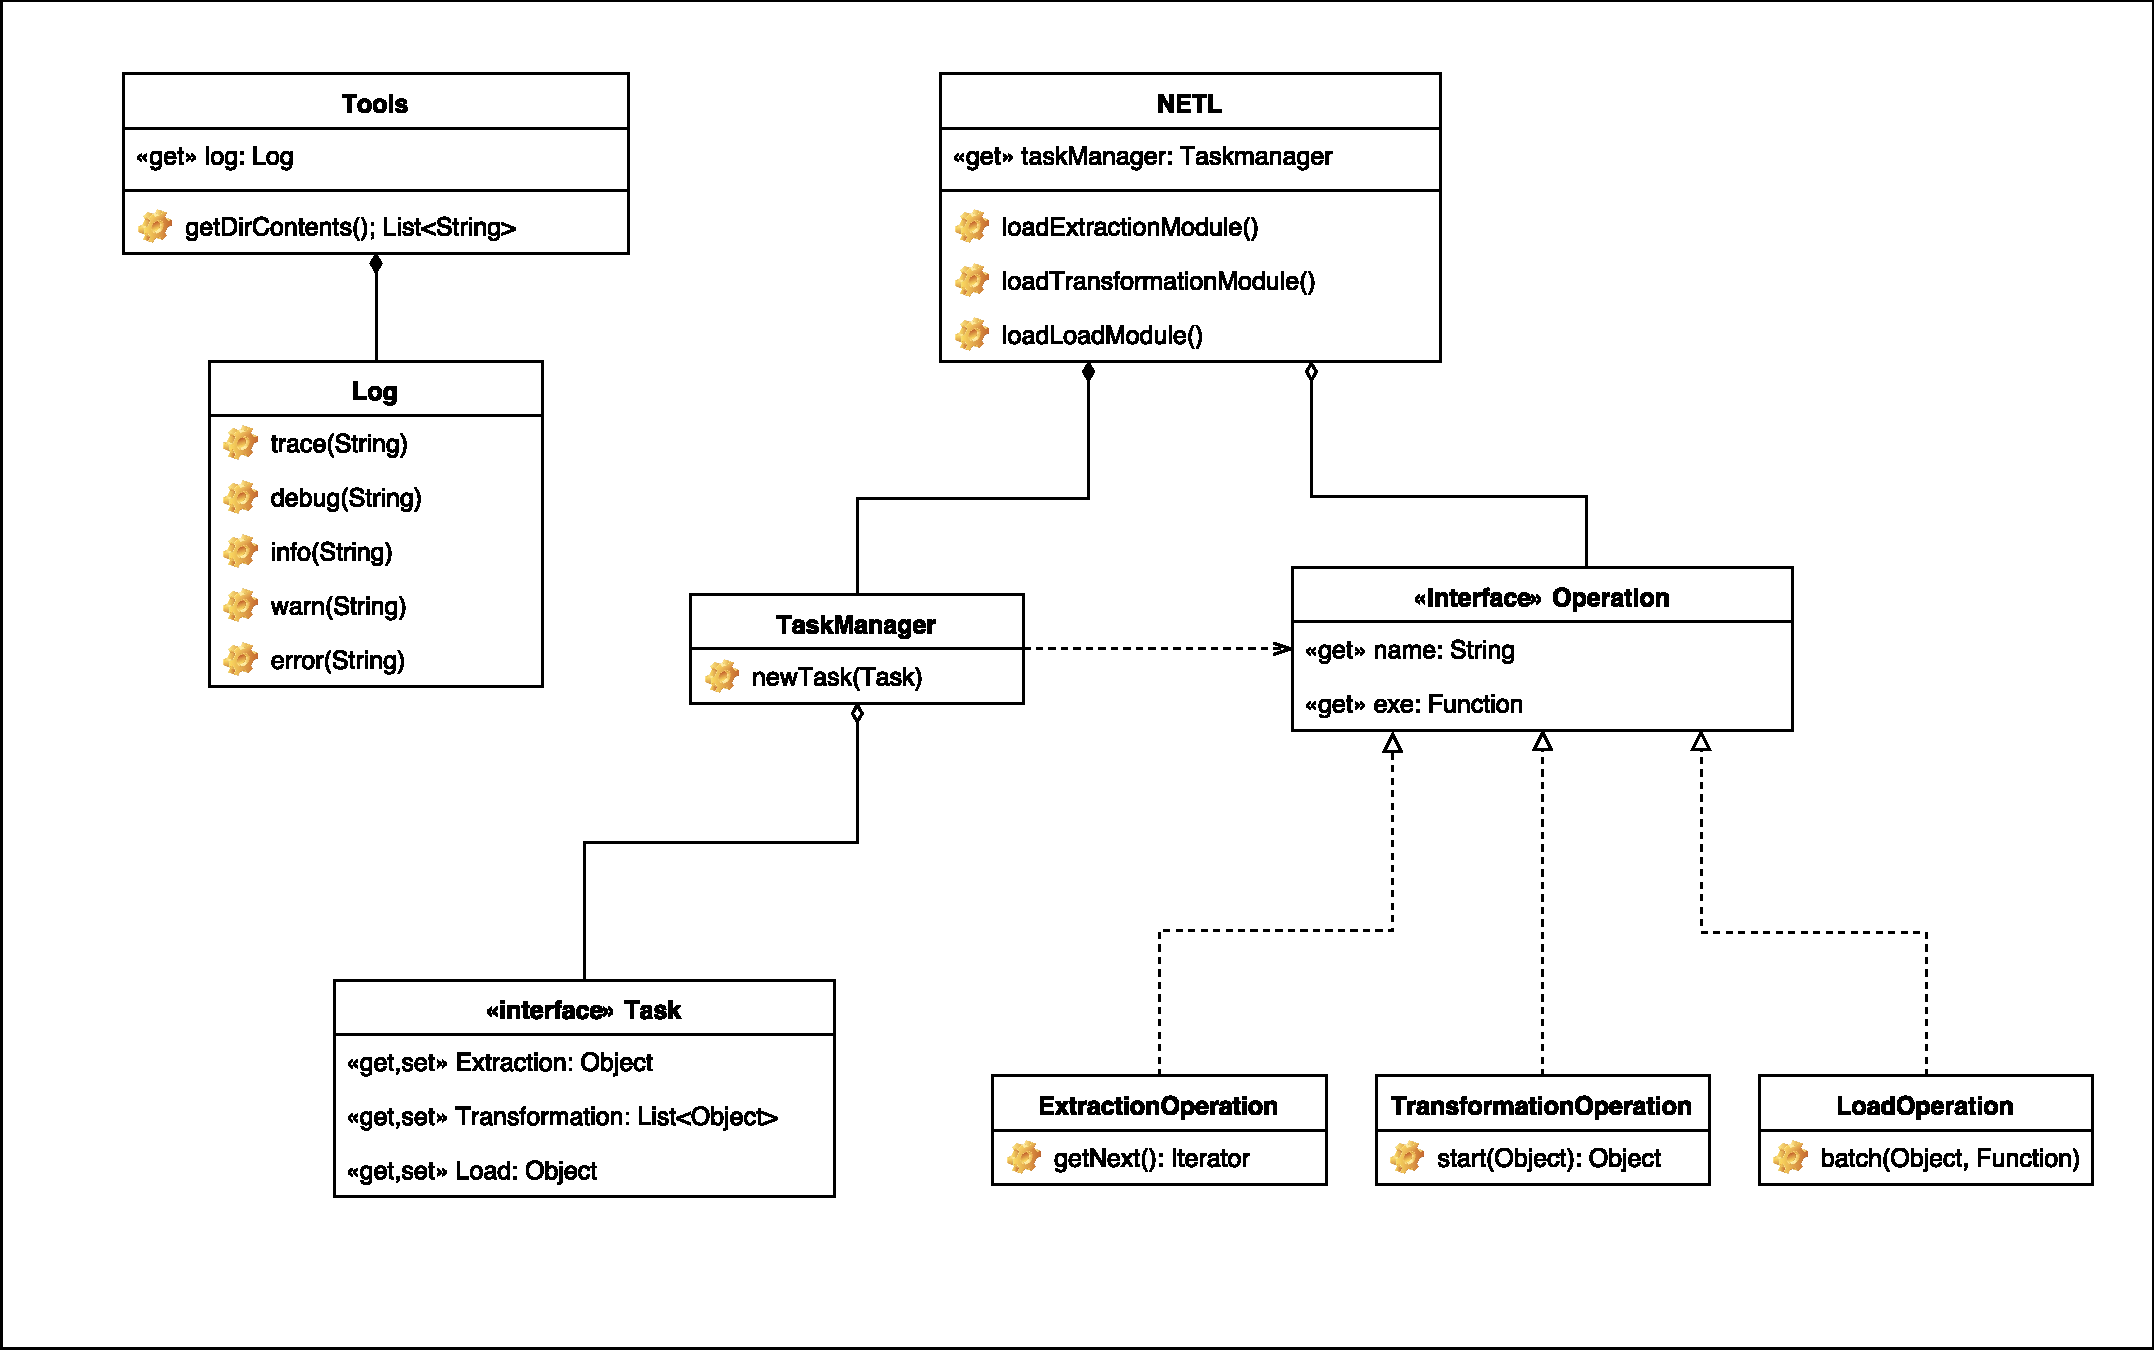
\includegraphics[scale=0.4]{./resources/figures/netlUML}
    \caption[nETL]{nETL}
    \label{nETL}
\end{figure}

Figure \ref{nETL} shows a potential architecture for a configurable component-based ETL tool. The intention of the framework is that it works on the basis of a pipeline of tasks. The framework itself is quite lightweight and comprises just the NETL, TaskManager and general purpose 'Tools' classes. For the purposes of this thesis, the framework as described by Figure \ref{nETL} has been prototyped in node.js. \textit{JavaScript} is a suitable language to prototype this application for a number of reasons:

\begin{enumerate}
    \item It has a very succinct API making it fast to write code in (i.e. it is a highly abstracted language similarly to Ruby or Python)
    \item But unlike Ruby or Python (and other high level languages), it is opinionated in that it handles IO asynchronously by default
    \item The \textit{JavaScript} implementation of object-orientation is appealing (to some developers at least)
    \item And working and learning \textit{JavaScript} is very much in line with the spirit of CouchDB and the web in general
\end{enumerate}

nETL is primarily a task-managing application, and as such, the TaskManager class is effectively the core of the application and has been implemented via the following:

\begin{minted}{javascript}
function TaskManager(extractions, transformations, loads) {
    this.tasks = {};
    this.extractions = extractions;
    this.transformations = transformations;
    this.loads = loads;
};
TaskManager.prototype.newTask = function(task) { /* ... */ };
\end{minted}

The application itself is intended to be singleton instance of \mintinline{javascript}{class NETL{}}, which provides an interface to \textit{TaskManager}, and modular extraction/transformation and load operations. Singleton's are typically implemented via the modular pattern in JavaScript, which is typically how libraries are delivered to users by package managers and invoked by \mintinline{javascript}{var library = require('library-name')();}:

\begin{minted}{javascript}
module.exports = function() {
    const _extractions = {};
    const _transformations = {};
    const _loads = {};        
    const _taskManager = new TaskManager(_extractions, _transformations, _loads);
    function _loadExtractionModule(extractionOperation){};
    function _loadTransformationModule(transformOperation){};
    function _loadLoadModule(loadOperation){};
    return {
        taskManager: _taskManager,
        loadExtractionModule: _loadExtractionModule,
        loadTransformationModule: _loadTransformationModule,
        loadLoadModule: _loadLoadModule
    };
};
\end{minted}

To achieve batches loading, \textit{JavaScript} generators are are used. As described by \cite{mozillaGenerators}, \textit{JavaScript} generators allow for quickly implementing arbitrary iterators, including iterators over generated iterators. Using open source code provided by \cite{bower16}, nETL makes use of a generator function iterate of the lines of a file, and then a higher level generator to iterate over results of the line generator to produce \textit{batches} of data that are worked through the ETL pipeline.

\begin{minted}{javascript}
/**
 * Generates lines from a flatfile
 * @yield {string} returns a single line from a flatfile
 */
function* _readLines() {
    while (pointer < filesize) {
        yield lineBuffer;
    };
};

/**
 * Generates batches of lines
 * @yield {Object[]} An array of lines
 */
function* getBatch () {
    let data = [];
    for (0..batchSize) {
        data.push(lineExtraction.getNext());
    };
    yield data;
};

// Generate lines
var lineReader = _readLines();

// Generate batches of lines
var batch = getBatch.next();
\end{minted}

Transformations are then applied to batches of lines, with the result passed to a loading function. The loading function is implemented asynchronously due to the time-cost involved when using IO (and specifically using network IO as possible with CouchDB). As batches are successfully loaded, a new batch is extracted for processing via recursion.

\begin{minted}{javascript}
(function doEtlTask(self) {
    var payload = [];

    // Extract
    batch = batchExtraction.next();
    if (batch.done) return;

    // Apply transformations
    transformations.forEach(function(t) {
        batch = t.transform(batch);
    });
    payload = batch;

    // Load
    load.batch(payload)
        .then(function(msg) {
            doEtlTask(self);
        });
})();
\end{minted}